\documentclass[a4paper,10pt]{article}
\usepackage[utf8x]{inputenc}
\usepackage{graphicx}
\usepackage{pgf}
\pgfdeclareimage[height=1cm]{myimage}{p1_q1.png}


%opening   
\title{ \textbf{Universidade de Brasília -- Faculdade do Gama \\ Sistemas embarcados \\ Lista 1 }}
\date{}

\begin{document}
\maketitle

\paragraph{}
\textbf{Atenção:} Esta lista tem por objetivo relembrar conceitos de ponteiro e aguçar a compreensão sobre o tema. Esta é uma lista opcional e 
\textbf{não} será atribuído qualquer ponto adicional pela mesma, sendo indicada para aqueles alunos que desejam aprimorar os seus conhecimentos.
Esta lista tem como meta:
\begin{itemize}
 \item Melhorar a compreensão sobre os ponteiros em C.
 \item Relembrar conceitos básicos da linguagem C, como abertura de arquivos, manipulação de dados, dentre outros. 
 \item Fornecer novas ferramentas para os alunos.
\end{itemize}
Para o melhor aproveitamento do aluno, recomenda-se que o mesmo realize uma pesquisa sobre cada questão antes de tentar responde-la.

\section{Exercícios de revisão}

\begin{enumerate}
 \item Faça um algoritmo que calcule e imprima o tamanho em \emph{bytes} de um tipo de dados usando aritmética de ponteiros. Crie um ponteiro para cada 
      um dos tipos: \emph{float}, \emph{double}, \emph{int}, \emph{short}, \emph{long} e \emph{char}. Analise cuidadosamente os diferentes resultados.\\
      \textbf{Dica:}Comece a verificar os tamanhos partindo do \emph{char} e recomenda-se utilizar o resultado obtido como base para os demais. Por fim 
	recomenda-se verificar o tamanho dos tipos ponteiros utilizando a macro sizeof(ex.:char *, float *, void *).
 \item Um IP (\emph{Internet Protocol}) nada mais é que uma identificação de um dispositivo em uma rede local ou pública. Na sua versão 4, este é composto 
      por um endereços de até 32 bits. Faça um algoritmo que, utilizando ponteiros, crie um número IP a partir de 4 bytes lidos de um array de char. 
      Um número IP é um inteiro, onde cada byte que compõe o inteiro armazena um dos campos do IP (usar apenas ponteiros).\\
      Ex.: IP de uma máquina da FGA: 164.41.33.152\\
	  char fields[] = {152, 33, 41, 164};\\
	  Número inteiro que representa o IP:\\
	  Byte 0 = 152 // 0x98 em hexa\\
	  Byte 1 = 33 // 0x21\\
	  Byte 2 = 41 // 0x29\\
	  Byte 3 = 164 // 0xA4\\
	  ou IP = 0xA4292198\\
      Observação: Preste atenção ao total de bytes de cada tipo primitivo da sua máquina (o exercício anterior é útil neste sentido) e ao tipo de 
      organização da sua arquitetura (\emph{little ending ou big ending}).
      \textbf{Dica:} Utilize tipos sem sinal e inicialize os valores iniciais. 
 \item O formato de imagem PGM (\emph{Portable GreyMap}) é um padrão \emph{bitmap} que contém somente quatro linhas de cabeçalho, dados armazenados como unsigned 
      char fornecendo no máximo uma escala de cinza de 256 níveis. A estrutura geral do PGM é constituída de:\\
      \begin{itemize}
       \item Linha 1: Contém a assinatura do arquivo da imagem e identificador do arquivo PGM.
       \item Linha 2: É uma linha de comentário.
       \item Linha 3: Fornece informações sobre o número de linhas e colunas de dados armazenados em um arquivo.
       \item Linha 4: Especifica o nível máximo de cinza contido na imagem.
      \end{itemize}
      Um exemplo da estrutura de uma imagem no formato PGM:\\
	\\P5 \\
	\#FGA\/SEM imagem gerada Ver.1.0 (0) \\
	10 10 \\
	255 \\
	0 1 2 3 4 5 6 7 8 9 10 11 12 13 14 15 16 17 18 19 20 21 22 23 24 25 \\
	26 27 28 28 30 31 32 33 34 35 36 37 38 39 40 41 42 43 44 45 46 47 \\
	48 49 50 51 52 53 54 55 56 57 58 59 60 61 62 63 64 65 66 67 68 69 70 \\ 
	71 72 73 74 75 76 77 78 79 80 81 82 83 84 85 86 87 88 89 90 91 92 93 \\
	255 255 255 255 255 255 \\
      Um efeito muito comum que costuma-se dar a esta imagem é o chamado negativo. Este faz com que a cor de cada pixel da imagem original se 
      transforme na cor inversa (por exemplo, um pixel branco se transforma em preto), a cor inversa é o valor da subtração entre 255 e o valor 
      do pixel. Com base nas informações dadas, faça um programa que leia uma imagem no formato PGM, tire o negativo dela e salve-a como uma nova
      imagem.
  \item É comum que no processo de codificação sejam criadas funções para trabalhar com um determinado tipo nativo (por exemplo, \emph{int}), 
      contudo conforme o código passa a crescer surge a necessidade que tal função também trabalhe com outros tipos nativos. Como alternativa muitos 
      programadores replicam o trecho de código com o novo tipo ou buscam alguma solução que exige a implementação de mais código. Neste contexto 
      crie uma programa que receba um vetor como parâmetro e um valor chave para ser procurado dentro deste vetor. Faça com que esta função aceite 
      qualquer tipo de vetor, por exemplo, ela deve aceitar um vetor de \emph{int} ou \emph{double} sem precisar ser alterada. Use no máximo cinco 
      parâmetros e de como retorno em caso de sucesso na busca o valor da posição no vetor ou -1 no caso de nada ser encontrado. (Ignore o caso da 
      chave ser repetida, a primeira chave encontrada deve ser retornada).
      \textbf{Dica:} Utilize o referências do tipo \textbf{void}.
 
 \item \textbf{Desafio:}
      Vetores são exemplos de estruturas de dados simples e suportadas nativamente pela maiorias das linguagem de programação. Este tem duas  
      característica fundamentais: a necessidade de se conhecer previamente o seu tamanho inicial em tempo de compilação (ex.: \emph{int} num[2]) e 
      ter os seus elementos armazenados na memória de forma sequencial (isto garante o acesso imediato a um elemento). Contudo é comum termos 
      situações em que tais características não são desejáveis, como por exemplo em casos que não sabemos antecipadamente o tamanho total do vetor 
      em tempo de compilação, ou em casos menos comuns onde temos pouca memória contiguá disponível inviabilizando que um vetor caiba
      na memória sequencialmente. Uma possível solução para este problema é a chamada lista encadeada, que é uma estrutura composta por nós, 
      onde cada nó tem uma informação e um ponteiro para o próximo elemento da lista. Conhecido o primeiro elemento da lista, é possível acessar os 
      demais. Veja a figura abaixo mostrando vários nós com informação e apontando para outro nó:

\begin{figure}[ht]
 \center
 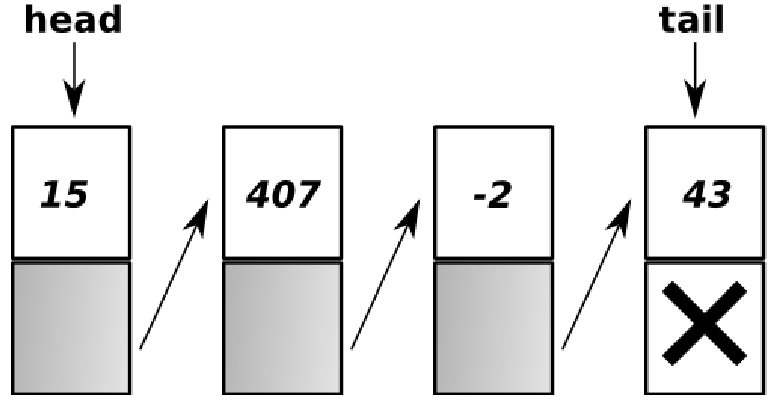
\includegraphics[width=10cm]{imagem/inserir_final_lista.png}
\end{figure}

      Para trabalhar com uma lista encadeada é preciso pelo menos duas estruturas, sendo a primeira referente ao nó (contém o valor de 
      interesse e a referência para o próximo nó) e a segunda a lista (Esta contém um nó referenciando ao primeiro elemento da lista e outro
      referenciando o último elemento). Além destas estruturas é necessário implementar funções de suporte que utilizaram esta estrutura e darão 
      significado a lista, como por exemplo funções para adicionar elementos na lista e remove-los. Com base nestas informações e na recomendação de 
      uma pesquisa sobre o tema, execute os passos abaixo para construir uma lista encadeada de inteiros.
  
  \begin{itemize}
   \item Crie um arquivo chamado ``node.h'', um arquivo chamado ``node.c'' e um chamado teste.c. 
   \item Abra o arquivo \emph{node.h} e faça os ajustes padrão para um arquivo .h. Defina uma estrutura onde o primeiro elemento seja 
	um tipo \emph{int} (a informação do nó) e o segundo seja um ponteiro para o próximo nó. \textbf{Observação:} O ponteiro para o próximo 
	nó será o tipo do tipo da estrutura que esta sendo criada. \\Exemplo: struct \_minhaStruct *next;
   \item Crie uma estrutura contendo dois elementos, sendo que ambos são referências do tipo da estrutura criada no passo anterior. Esta será 
	a estrutura da lista e recomenda-se que os dois elementos tenham nomes semelhantes a \emph{header} e \emph{tail}.
   \item No arquivo .h defina protótipos para as seguintes funções: função que cria a lista, que adiciona um elemento na fila (recomenda-se algo com 
	a terminologia \emph{push}), outra para remover um elemento do final da fila, uma para imprimir os dados da fila e por fim uma para 
	excluir a fila.
   \item No arquivo \emph{node.c} insira as funções criadas no arquivo \emph{node.h} com a intenção de implementa-las. 
   \item Implemente a função que criará a lista na memória. Para isto utilize a função \emph{malloc, calloc} ou algo semelhante. \textbf{Dica: 
	busque realizar uma pesquisa sobre tais funções}.
   \item Implemente a função que insere um elemento no início da lista. Preste atenção para o caso em que a fila não foi iniciada e para o caso 
	em que ela não possui nenhum elemento, ou seja, o caso da lista criada estar vazia.
   \item Implemente a função que remove um elemento da lista. Leve em consideração o caso em que o elemento a ser removido é o último e o caso 
	da lista estar vazia.
   \item Implemente a função que exclui a fila da memória.
   \item Implemente a função que imprime toda a lista. Para isto colete a referência para o primeiro elemento da lista (\emph{head}) e faça um 
	loop em que verifique se o nó atual esta \emph{null} (caso do último elemento). Caso o no não esteja vazio passe para o próximo elemento 
	da fila.
   \item Abra o arquivo teste.c e crie uma lista encadeada por meio da função de criação da lista (que você já criou). Em seguida crie um pequeno 
	menu contendo as seguintes opções: 1 - Adicionar um inteiro, 2 - Remover um inteiro, 3 - Mostrar a lista e 4 - Sair do programa. Cada 
	opção deverá atuar sobre a lista.
  \end{itemize}

\end{enumerate}

\end{document}
